\section{First Week: Core of Java}

\subsection{Orientation}

In the first day of my internship, the company introduced itself by 1-hour orientation. In the orientation, general information about company and internship programs was provided. Additionally, information about management systems, personal data protection law (KVKK), and occupational health and safety (OHS) are given.

After the orientation, I met with my team. Firstly, our mentor introduced himself, then, everyone do so. General internship schedule was shared and our responsibilities in our internship are stated. Our main responsibility was attending the programs/classes on time.

\subsection{Environment Setup and First Program}

Since we will have been using Java during internship, necessary development environments should be introduced and installed. After setup of Java SDK was shown, we discussed the coding environment. IntelliJ IDEA is suggested by our mentor and the setup of it was shown. 

After we discussed what a software is and how it works on a computer, programming languages, we talked about the history and working structure of Java. Then, we continued by creating the first project on IntelliJ IDEA, we coded the first program, the classic \textit{Hello World!}.

\subsection{Introduction to Java}

We started with the basics learned/taught while learning a new programming language in the ordinary way. The four days of the first week was about the basics and core concepts about Java. Since syntax and basic concepts of Java are quite similar to C and C++, understanding the topics that were covered was not that hard for me in the beginning of the week. Even though I was learning some tricks about Java and coding, generally, it was like I was learning syntax of Java.

While learning the concepts and basics, we usually practised about them. Normal process was that after we first coded the exercise, we examined the sample solutions that had been coded by other team members. If there was an error in someone's code or someone could not understand a part of the example, we had learned together by looking at those codes. This approach has been quite useful for me at times because examining codes of other people really helps the learning phase.

\subsubsection{Basics of Java}

We started by talking about comments, identifiers, escape sequences, data types, operators, basic input and output, conditions and loops. While learning these, data types were, most probably, the most complicated part. Although I was familiar with the terms ``call-by-value'' or ``call-by-reference'', I believe that in order to gain a deep understanding of data types in Java language, time needs to be devoted on them. Strings in Java, for example, can be considered as both primitive and reference data types.

Then, arrays whose preferred syntax in Java is different than C++, type casting, and variable length argument lists came up. In arrays and type casting, they works almost same in both Java and C++. Even though it is included other languages, it was the first time I heard of the ``variable length argument lists'', which is used for unspecified number of arguments. 

Since strings have special positions in some languages and I believe Java is one of them. Strings can be confused because they can behave like both primitive and reference types. Also, I learned about \textit{StringBuffer} and \textit{StringBuilder} which are basic classes to construct strings and add some functionality to strings. Even though I knew what exceptions are, I did not practised much. Actually, I can say that I learned how it really works and is used in this internship.

We also talked about advanced Java IO as well as the concept of ``serialization''. I believe that although it is a little bit harder than other languages I use such as \texttt{Python}, file handling is a little bit more flexible in \texttt{JAVA} thanks to variety. There are several classes to make the file reading and writing easier.

After these basics, some advanced features such as enumerations, interfaces, abstract and generic classes are disccussed. Although these were not new to me, I barely knew what they are and why we use them but thanks to exercises I understood these. Interfaces was a little bit tricky for me because it was the first time I encountered such thing. Then, an unfamiliar topic came up: wildcards about which I was not know anything but useful as well. 

\subsubsection{Collections in Java}

From the courses I have taken, I know the some data structures. In this part, I learned that Java provides a variety of collections whose implementations are different under the hood. The collections that are in the figure below is discussed. 

% Taken from https://facingissuesonit.com/2019/10/15/java-collection-framework-hierarchy/
\begin{figure}[h!]
  \centering
  \copyrightbox[b]{
    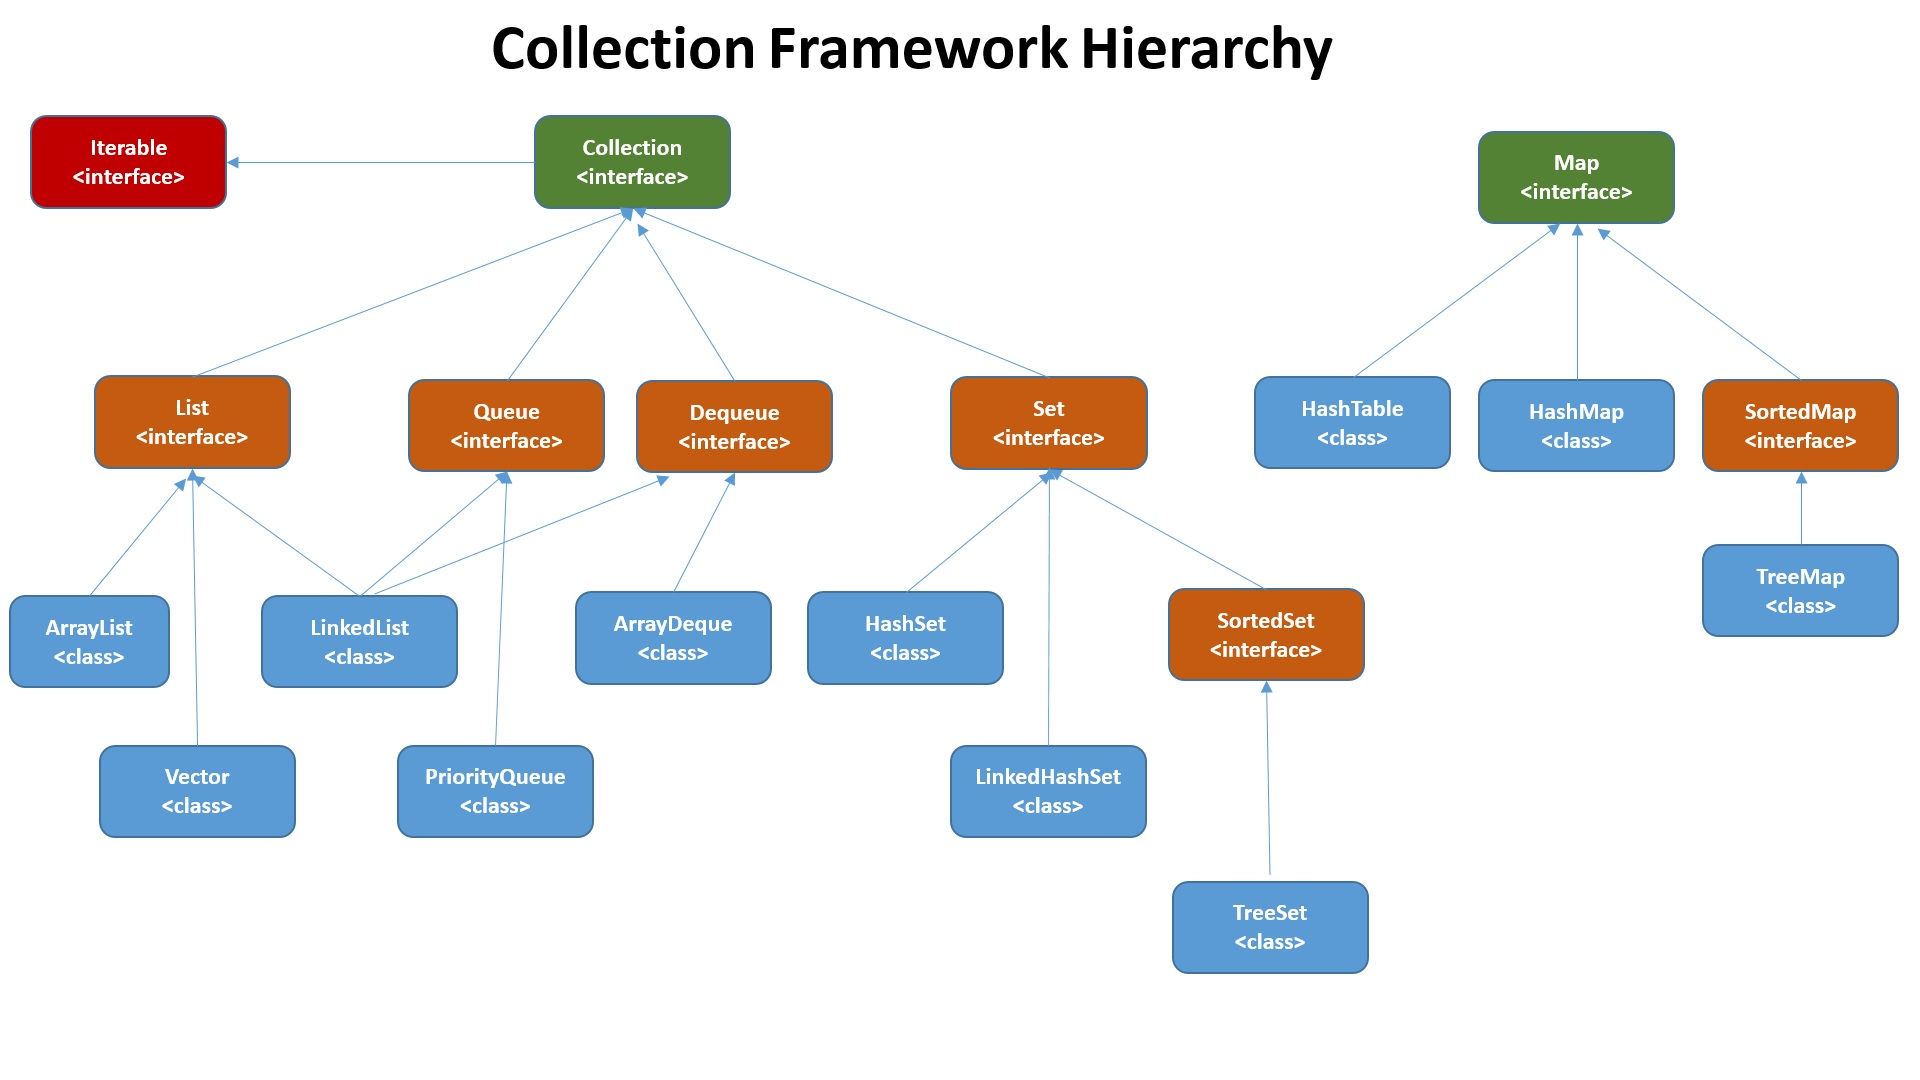
\includegraphics[width=\linewidth]{img/java-collection.jpg}
  }{
    Source: \url{https://facingissuesonit.com/2019/10/15/java-collection-framework-hierarchy/}
  }
\end{figure}

Also, \texttt{hashCode()} and \texttt{equals()}, important methods for these collections to work properly, were discussed. It was shown that what they are and why we use them.

\subsubsection{OOP}

In this part, basics and prenciples of the Object Oriented Programming (OOP) are covered.

We started by talking about the basics such as scopes, constructors, access modifiers, setter and getter methods, method overloading, static methods. Since I was familiar to concepts from the CENG 242: Programming Language Concepts, I did not have hard time about these concepts.

After the basics, we moved into the prenciples. We started with inheritance and class hierarchy. In here, I learnt that Java does not support multiple inheritance as well as what superclasses and subclasses are. Furthermore, behaviours of some concepts, such as access modifiers and constructors, in inheritance are discussed. Also, other prenciples abstraction, encapsulation and polymorphism are covered but I did not learn new information.

\subsubsection{JavaBeans and JDBC}

The last day of the week, when we got out of the basics of Java and learned databases and database connections by using Java, was really a day that I learned new information and challenged me for the first time in this week.

We started by talking the JavaBeans, which is basically a standard. By reading learning and reading about JavaBeans, I learned that many things are standardized in Java and implementations are competed instead of the standards, which makes the reason why Java is quite preffered in corporate area clear.

Since we will have needed to add some dependencies and Maven was going to used in our projects, we talked avbout Maven, a build automation tool, and installed it in addition to MySQL, which were going to be used as database. After the installations and the adjusments of environment, we dived into the Java Database Connectivity (JDBC), which is Java API that mainly manages connecting to a database. Connecting to a database, executing queries, using of ``\texttt{Statement}'', ``\texttt{ResultSet}'' and ``\texttt{PreparedStatement}'' which are basically used to sending SQL statements to databases, and transaction management.


\subsection{Git \& Bitbucket}

To our use during the internship, we were provided a Bitbucket account. We were asked to use Git and ``\textit{push}'' our codes to Bitbucket. Since we were asked to use Git, the basics and basic usage of Git and Bitbucket was shown. 


% \noindent Additionally, the OOP examples are done:
% \begin{itemize}
%   \item \textbf{ExampleThePen:} Constructors, Set and Get methods, Shadowing, \texttt{static} keyword.
%   \item \textbf{ExampleBusReservation:} Constructors, Set and Get methods, Shadowing, \texttt{static} keyword, Enumerations.
% \end{itemize}

% Example of the topic: \texttt{ExampleException}, Example IO

% The example \texttt{ExampleOccurrencesOfWords} is done.

% Some days, Some friends was talking about design patterns. In the third day of my internship, two people talked about two different design patterns, which are \textit{Adepter} and \textit{MVC} design patterns.

% New projects are opened after Inner Class part: \texttt{JIP-JDBC}.

% After these concepts are disccussed, example named \texttt{ExamplePenRevisited} is done.

% We have done the example named \texttt{ExampleInterfacePen}.